\documentclass[12pt,a4paper,oneside,dvipsnames,table,svgnames,skins,theorems]{report}

\usepackage{ProfCollege}
%\usepackage[nominted]{ProfLycee}
\usepackage[tp]{tmbase} %pour le moment placé dans la racine du .tex ... !




\ordi{fixe} %pour fichier image
\matierechap{m} %m pour maths, pc pour physique chimie, rien pour vierge
\version{1} %1 : PROF   2: ELEVE sans corrigé  3: corrigé des exos sans le cours
\setcounter{chapter}{0} %compteur de chapitre

\ifportable

\graphicspath{{C:/Users/Thomas/latex nas/images/}} %chemin du fichier image
\fi
\iffixe
\graphicspath{{C:/Users/Thom/Documents/latex nas/images/}} %chemin du fichier image
\fi

%\author{TP}
\author{Devoir 3} %mettre ici non pas l'auteur mais la partie en haut à gauche de l'encadré


%\newcolumntype{C}{>{\centering\arraybackslash}X}
%\renewcommand{\tabularxcolumn}[1]{>{\arraybackslash}m{#1}}
\begin{document}

\setcounter{chapter}{2}

\chapter{ Fonction log  }


\begin{center}
\mybox{
Calculatrice autorisée; Formulaire autorisé.
}
\end{center}




\Opensolutionfile{mycor}[ficcorex]


\exo{} Le cola est une boisson sucrée dont la concentration en ions \chemfig{H_3 O^{+}} est : $c=\SI{0.00316}{\mol\per\liter}$.\\
Le pH d'une solution se calcule par la formule $pH = -\log c$ avec $c$ la concentration en ions \chemfig{H_3 O^{+}}  en \si{\mol\per\liter}.

\begin{center}
\includegraphics[scale=0.4]{ph.png}
\end{center}
\vspace{-0.5cm}
\textbf{Calculer le pH du cola et préciser s'il est acide ou basique.
}
\begin{correction}
On calcule $pH= -\log 0.00316 = 2.5$ ce qui fait du cola une boisson très acide.
\end{correction}
\finexo
%\vspace{-0.5cm}
%\exo{} On a relevé durant 6 mois le nombre de passagers  sur une ligne de train "low cost" :
%\vspace{0.1cm}
%
%\begin{tabularx}{\textwidth}{|C|C|C|C|C|C|C|}
%\hline
%Mois & Février & Mars & Avril & Mai & Juin & Juillet \crh
%Rang & 1 & & & & & \crh
%Passagers & 1220 & 1400 & 1610 & 1815 & 2040 & 2385 \crh
%\end{tabularx}
%
%\problematique{Déterminer le mois pour lequel on atteindra la capacité maximale de la ligne à savoir 3000 passagers.}
%
%\begin{correction}
%Le nuage de point et la droite de régression : $R^2 = 0.9874$ $f(x)=227.14x+950$
%\begin{center}
%\begin{tikzpicture}[scale=1.4]
%
%
%\begin{axis}[axis x line=bottom, axis y line = left, grid=major, xlabel={Rang}, ylabel={passagers},
%xmin=0, xmax=12, ymin=1200, ymax=4000, xstep=1]
%
%\addplot[forget plot,only marks] table[x=rang,y=passagers]{stats2var4.txt};
%\addplot[no marks, color=red] table[y={create col/linear regression={y=passagers}}] 
%    {stats2var4.txt};
%\addlegendentry{%
%$y=\pgfmathprintnumber{\pgfplotstableregressiona} \cdot x
%\pgfmathprintnumber[print sign]{\pgfplotstableregressionb}$}
%\addplot[no marks,red,domain=6:11]{\pgfplotstableregressiona*x+\pgfplotstableregressionb};
%\addplot[only marks, blue, mark=x] (9.02,3000);
%\end{axis}
%\end{tikzpicture}
%\end{center}
%Par une lecture graphique on atteint 3000 passagers au rang 9 ce qui donnerait octobre.
%
%\end{correction}
%\finexo
\vspace{0.1cm}

\exo{} Calculer, en détaillant, la valeur de $\log 726$.
\vspace{0.2cm}

On donne : $\log 2 = 0.3$ , $\log 3 = 0.48$, $\log 5 =0.7$, $\log 7 = 0.85$ et $\log 11 = 1.04$.
\begin{correction}
On peut démontrer que $\log 726 = \log 3 + \log 2 + 2\log 11 \approx 2.86$
\end{correction}

\finexo
\vspace{0.1cm}
%\newpage

\exo{} On donne plusieurs distances mesurées entre des objets :
\begin{itemize}
\item La distance Terre-Lune : \SI{4.0e5}{\kilo\meter}
\item La distance Terre-Soleil : \SI{1.5e8}{\kilo\meter}
\item La distance Paris - Marseille : \SI{800}{\kilo\meter}
\item La distance Saint Etienne - Lyon : \SI{65}{\kilo\meter}
\item La distance Salle de Maths - Cantine : \SI{250}{\meter}
\item La distance entre deux élèves : \SI{2}{\meter}
\end{itemize}
\vspace{0.2cm}

\begin{enumerate}
\item Citer une raison pour laquelle ces distances ne peuvent être simplement représentées sur un repère gradué en l'état.
\item Proposer une méthode permettant de transformer les données pour les représenter sur un repère.
\item Convertir toutes les données dans la même unité (de votre choix, il est judicieux de tout placer en \si{\meter})
\item Mettre en oeuvre votre méthode à la question 2 pour représenter, sur votre copie, les données sur un graphique de taille pertinente. On détaillera la démarche.

\end{enumerate}
\begin{correction}
\begin{enumerate}
\item La différence d'échelle entre la plus grande et la plus petite est trop importante.
\item On pourrait tout exprimer sous la forme d'un logarithme décimal et représenter ensuite sur une échelle logarithmique les grandeurs.
\item Conversions en mètres :
\begin{itemize}
\item La distance Terre-Lune : \SI{4.0e5}{\kilo\meter} = \SI{4.0e8}{\meter}
\item La distance Terre-Soleil : \SI{1.5e8}{\kilo\meter} = \SI{1.5e11}{\meter}
\item La distance Paris - Marseille : \SI{800}{\kilo\meter} = \SI{800e3}{\meter}
\item La distance Saint Etienne - Lyon : \SI{65}{\kilo\meter} = \SI{65e3}{\meter}
\item La distance Salle de Maths - Cantine : \SI{250}{\meter}
\item La distance entre deux élèves : \SI{2}{\meter}
\end{itemize}
\item Tableau :
\end{enumerate}
\vspace{0.5cm}


\renewcommand{\arraystretch}{2}

\begin{tabularx}{\textwidth}{|C|C|C|C|C|C|C|}
\hline
Grandeur & Terre Lune & Terre Soleil& Paris Marseille & St Etienne - Lyon & Salle de maths - Cantine & Eleves \crh
{\footnotesize Distance $d$}  (\si{\meter}) & \SI{4.0e8}{} &\SI{1.5e11}{} &\SI{800e3}{} & \SI{65e3}{}&  \SI{250}{} & \SI{2}{}\crh
 $\log d$ &8.6 &11.2 &5.9 &4.8 & 2.4 &0.3  \crh
\end{tabularx}

\begin{enumerate}[resume]
\item Cette échelle est plus réalisable sur une feuille que la précédente les valeurs étant comprises entre 0 et 12.
\end{enumerate}
\vspace{2cm}


\begin{center}
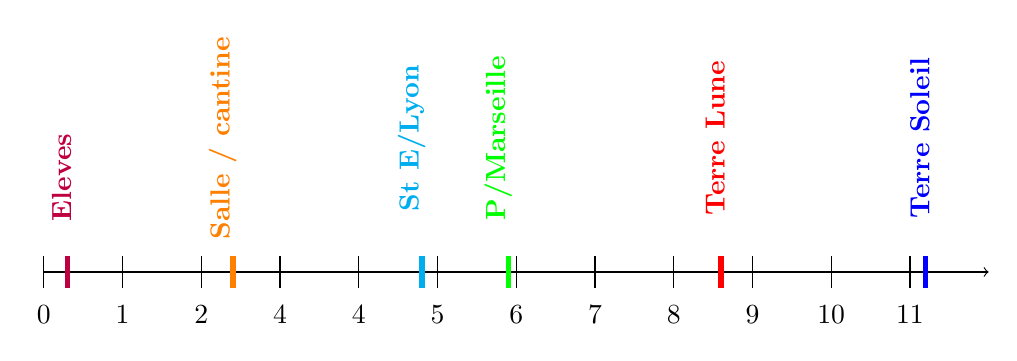
\begin{tikzpicture}
\draw[->] (-6,0)--(6,0);
\foreach \x/\y in{-6/0,-5/1,-4/2,-3/4,-2/4,-1/5,0/6,1/7,2/8,3/9,4/10,5/11}
{
\draw (\x,-0.2)--(\x,0.2) node[below=0.5cm]{\y};
}
\draw[color=red,line width=2pt] (2.6,-0.2)--(2.6,0.2)node[right=0.2cm,above=1.5cm,rotate=90]{\textbf{Terre Lune}};
\draw[color=blue,line width=2pt] (5.2,-0.2)--(5.2,0.2)node[right=0.2cm,above=1.5cm,rotate=90]{\textbf{Terre Soleil}};
\draw[color=green,line width=2pt] (-0.1,-0.2)--(-0.1,0.2)node[right=0.2cm,above=1.5cm,rotate=90]{\textbf{P/Marseille}};
\draw[color=cyan,line width=2pt] (-1.2,-0.2)--(-1.2,0.2)node[right=0.2cm,above=1.5cm,rotate=90]{\textbf{St E/Lyon}};
\draw[color=orange,line width=2pt] (-3.6,-0.2)--(-3.6,0.2)node[right=0.2cm,above=1.5cm,rotate=90]{\textbf{Salle / cantine}};
\draw[color=purple,line width=2pt] (-5.7,-0.2)--(-5.7,0.2)node[right=0.2cm,above=1cm,rotate=90]{\textbf{Eleves}};
\end{tikzpicture}
\end{center}

Cette échelle permet d'évaluer des ordre de grandeur (chaque unité est une puissance de 10).


\end{correction}
\finexo

%\exo{} Un produit est commercialisé en vente en ligne et semble être en perte de vitesse depuis quelques années. Ce produit est basé sur un principe actif : le lysozyme. On donne le tableau :
%\vspace{0.1cm}
%
%\begin{tabularx}{\textwidth}{|C|C|C|C|C|C|C|}
%\hline
%Année & 2015 & 2016 & 2017 & 2018 & 2019 & 2020  \crh
%Rang & 1 & & & & & \crh
%V (en milliers d'exemplaires) & 8224 & 4112 & 2056 & 1028 & 514 & 257 \crh
%\end{tabularx}
%
%\begin{enumerate}
%\item Préciser si les ventes diminuent ou augmentent au fil des années
%\item Détailler le principe de la méthode vue dans les statistiques à 2 variables pour estimer les ventes en 2021 et 2022.
%\item Mettre en œuvre cette méthode sur votre calculatrice.
%\item Expliquer pourquoi cette méthode ne convient pas dans cette situation.
%\item Recopier et compléter le tableau suivant : (les calculs ne sont pas demandés). Arrondir au centième.
%\end{enumerate}
%
%\vspace{0.1cm}
%
%\begin{tabularx}{\textwidth}{|C|C|C|C|C|C|C|}
%\hline
%Année & 2015 & 2016 & 2017 & 2018 & 2019 & 2020  \crh
%Rang & 1 & & & & & \crh
%$\log V$ & & & & & & \crh
%\end{tabularx}
%\vspace{0.3cm}
%
%Un élève a réalisé l'ajustement affine avec le second tableau et obtient :
%\begin{center}
%\includegraphics[scale=1]{dslog.png}
%\end{center}
%\begin{enumerate}[resume]
%\item Expliquer pourquoi dans cette situation l'analyse est utilisable.
%\item Par une résolution d'équation, déterminer $y_7$, qui correspond aux ventes pour l'année 2021.
%\end{enumerate}
%Cette valeur $y_7$ n'est pas le nombre de vente mais le $\log$ de $V_7$.
%\begin{enumerate}[resume]
%\item En utilisant la propriété adaptée, calculer $V_7$ et arrondir à l'unité.
%\item Par la méthode de votre choix (graphique ou équation), déterminer $y_8$ pour l'année 2022.
%\item Calculer $V_8$ et arrondir à l'unité.
%\item Sans justifier, selon vous en quelle année les ventes tomberont en dessous de 25 000 produits par an ?
%\item \textbf{Question bonus :  résoudre $V=25$ et déterminer précisément l'année.}
%\end{enumerate}
%
%\begin{correction}
%\begin{enumerate}
%\item Le tableau montre une diminution
%\item Compléter la ligne du rang, représenter le nuage de point correspondant au rang et aux ventes, tracer la droite d'ajustement, si le coefficient $R^2>0.9$ alors on peut utiliser ce modèle pour prévoir.
%\item Graphique :
%\begin{center}
%\includegraphics[scale=1]{nuageds.png}
%\end{center}
%\item Le $R^2$ est trop petit, la méthode de l'ajustement linéaire n'est pas correcte. On va essayer de faire un ajustement logarithmique.
%\item Tableau :
%\vspace{0.1cm}
%
%\begin{tabularx}{\textwidth}{|C|C|C|C|C|C|C|}
%\hline
%Année & 2015 & 2016 & 2017 & 2018 & 2019 & 2020  \crh
%Rang & 1 & 2& 3&4 &5 &6 \crh
%$\log V$ &3.92 &3.61 &3.31 &3.01 &2.71 &2.41 \crh
%\end{tabularx}
%\vspace{0.3cm}
%
%\item Avec le graphique, on voit le $R^2=1$ ce qui est parfait, on peut donc utiliser cette modélisation
%\item $y_7 = -0.0301 \times 7 +4.2161 = 2.11$
%\item $V_7=10^{2.11} = 129$ 
%\item Même méthode : $y_8 = 1.81$ et $V_8 = 10^{1.81} = 64$
%\item A ce rythme de diviser par deux en un an, on peut penser qu'il faudra encore deux ans soit en 2024
%\item Vérification : $ V = 25 \implies  y= 1.4 \implies 1.4 = -0.301x + 4.2161 \implies 1.4 - 4.2161 = -0.301x \implies x = \dfrac{-2.8161}{-0.301} = 9.4$ donc entre le rang 9 et 10 ce qui correspond à l'année 2023 et 2024. La prédiction était correcte. 
%\end{enumerate}
%\end{correction}
%\finexo
\vspace{0.5cm}



\newpage
\begin{center}Corrigé des exercices\end{center}
\setcounter{page}{1}
\Closesolutionfile{mycor}
\Readsolutionfile{mycor}

\thispagestyle{empty}



\end{document}